\chapter{Analýza existujících řešení}

\begin{chapterabstract}
Tato kapitola se zabývá rešerší existujících řešení. Pro rešerši byly zvoleny aplikace, které poskytují informace o výsledcích hlasování o návrzích zákonů. Aplikace byly nalezeny v rámci různých článků na internetu o aplikacích poskytujících informace o aktuálním politickém \linebreak dění, včetně informace o návrzích zákonů.
\end{chapterabstract}

\section{politiscope}

\begin{description}
	\item \textbf{Autor:} Android Politiscope Developer
	\item \textbf{Počet stažení:} více než 10 000
	\item \textbf{Analyzovaná verze:} 2.4 (26. 1., 2023)
\end{description}

\noindent Aplikace politiscope \cite{politiscope} dle popisu na Google Play poskytuje informace ohledně politickém dění ve Spojených Státech. Informace jsou objektivní a jsou podány v jednoduché formě. Aplikace poskytuje informace o politických reprezentantech a jejich hlasováních. Aktuální témata jsou barevně označena. Uživatelé mají možnost ukládat návrhy zákonů a sledovat průběh jejich hlasování. Uživatelé mají také možnost sledovat konkrétní politické reprezentanty. Návrhy zákonů jsou označeny tagy pro snazší vyhledání. U témat jsou oficiální sumarizace a odkazy na oficiální zdroje. Lze také sledovat průběh voleb a kampaní.

Aplikace čerpá data z API poskytuných z následujícíh zdrojů

\begin{itemize}
	\item prorepublica \cite{propublica} -- ProPublica je nezávislá, nezisková redakce.
	\item theunitedstates \cite{unitedstates} -- @unitedstates je projekt poskytující data ohledně Spojených Států veřejností a pro veřejnost.
	\item congress \cite{congress} -- Congress.gov je oficiální portál pro informace z Kongresu a orgánů státní správy Spojených Států.
	\item openfec \cite{openfec} -- OpenFEC je oficiální portál vlády Spojených Států.
\end{itemize}

\noindent Výše uvedené informace jsou čerpány čistě z popisu a screenshotů aplikace na Google Playi. Do aplikace se mi nepodařilo dostat. Pro přístup je potřeba zaregistrovat se a přihlásit se. Po registraci mě to však automaticky přesměruje na přihlášovací obrazovku, kde po zadání přihlašovacích údaju to pak píše, že účet se zadanými přihlašovacími údaji neexistuje. Aplikaci jsem testoval na dvou různých zařízeních a na obou se vyskytl stejný problém. Aplikace má přesto přes 10 000 stažení, a tudíž ve většině případech funguje. Tipuji, že problém souvisí s geografickou lokací mobilního zařízení. Na obrázcích \ref{fig:politoscope} lze vidět, jak aplikace vypadá.

\begin{figure}
	\centering

	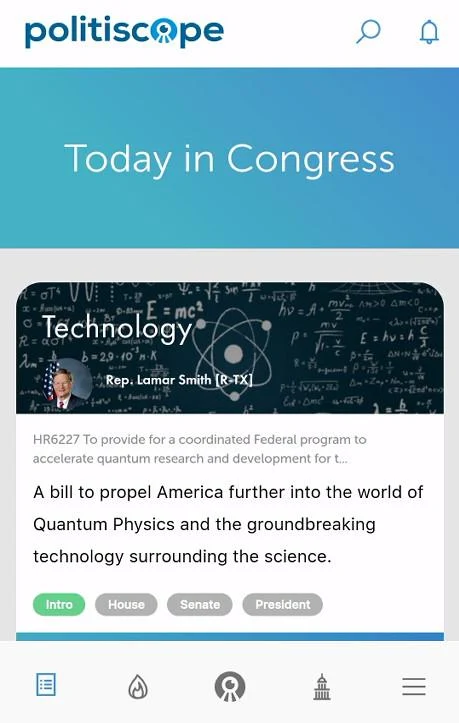
\includegraphics[width=0.4\linewidth]{politiscope}
	
\includegraphics[width=0.4\linewidth]{politiscope2}
	
	\caption{Android aplikace politiscope \cite{politiscope}}
	\label{fig:politoscope}
\end{figure}

\subsection{Zhodnocení}
Přestože se mi  aplikaci nepodařilo zprovoznit, stálo za to zahrnout ji do analýzy kvůli jejím funkčnostem. Další výhodou této aplikace je také přívětivé uživatelské rozhraní a fakt, že data získává z již existujících API.

\section{Congress}

\begin{description}
	\item \textbf{Autor:} Eric Mill
	\item \textbf{Počet stažení:} více než 500 000
	\item \textbf{Analyzovaná verze:} 4.9.2 (27. 1., 2023)
\end{description}

\noindent Aplikace Congress \cite{congress} dle popisu na Google Play poskytuje informace o politických reprezentantech a výsledcích jejich hlasování o návrzích zákonů ve Spojených Státech. Návrhy zákonů lze vyhledávat podle názvu.

Při spuštění aplikace uvidíme domovskou obrazovku, která obsahuje menu pro seznam politických reprezentantů, návrhů zákonů, výsledků hlasování, aktivit v rámci Kongresu, schůzek komisí \linebreak a seznam komisí. Na domovské stránce uvidíme také seznam nejnovějších návrhů zákonů. 

Obrazovka pro seznam politických reprezentantů obsahuje seznam aktuálně sledovaných politických reprezentatntů. Reprezentatny lze filtrovat podle státu, sněmovny a senátu. Na obrazovce konkrétního politického reprezentanta lze vidět jeho jméno, politickou stranu, příslušný stát, telefonní číslo, jak hlasoval, které zákony navrhoval, ke kterým komisím patří a odkaz na oficiální stránku s informacemi o něm. 

Obrazovka pro návrhy zákonů obsahuje seznam návrhů sledovaných uživatelem, seznam aktivních návrhů a seznam nových návrhů.

Na obrazovce pro výsledky hlasování lze vidět popis návrhu, výsledek hlasování \linebreak o návrhu, datum a čas hlasování, a údaj o tom, zda se hlasovalo ve Sněmovně nebo Senátu. Obrazovka s detailem návrhu zákona obsahuje výsledek jeho hlasování, počet hlasování \linebreak pro a proti, a počet lidí, kteří nehlasovali. Dále obsahuje informaci o tom, kolik lidí je potřeba být ve fyzické přítomnosti, aby hlasování bylo platné. Dále obrazovka obsahuje informaci \linebreak o tom, jak hlasoval který politik o daném návrhu.

Obrazovka pro události v kongresu obsahuje seznam událostí. Události jsou rozdělené podle toho, zda nastaly ve Sněmovně nebo v Senátu. 

Obrazovka pro schůzky komisí a obrazovka pro seznam komisí byly v době analýzy aplikace prázdné.

Na obrázcích \ref{fig:congress} lze vidět, jak aplikace vypadá.
 
\begin{figure}
	\centering
	
	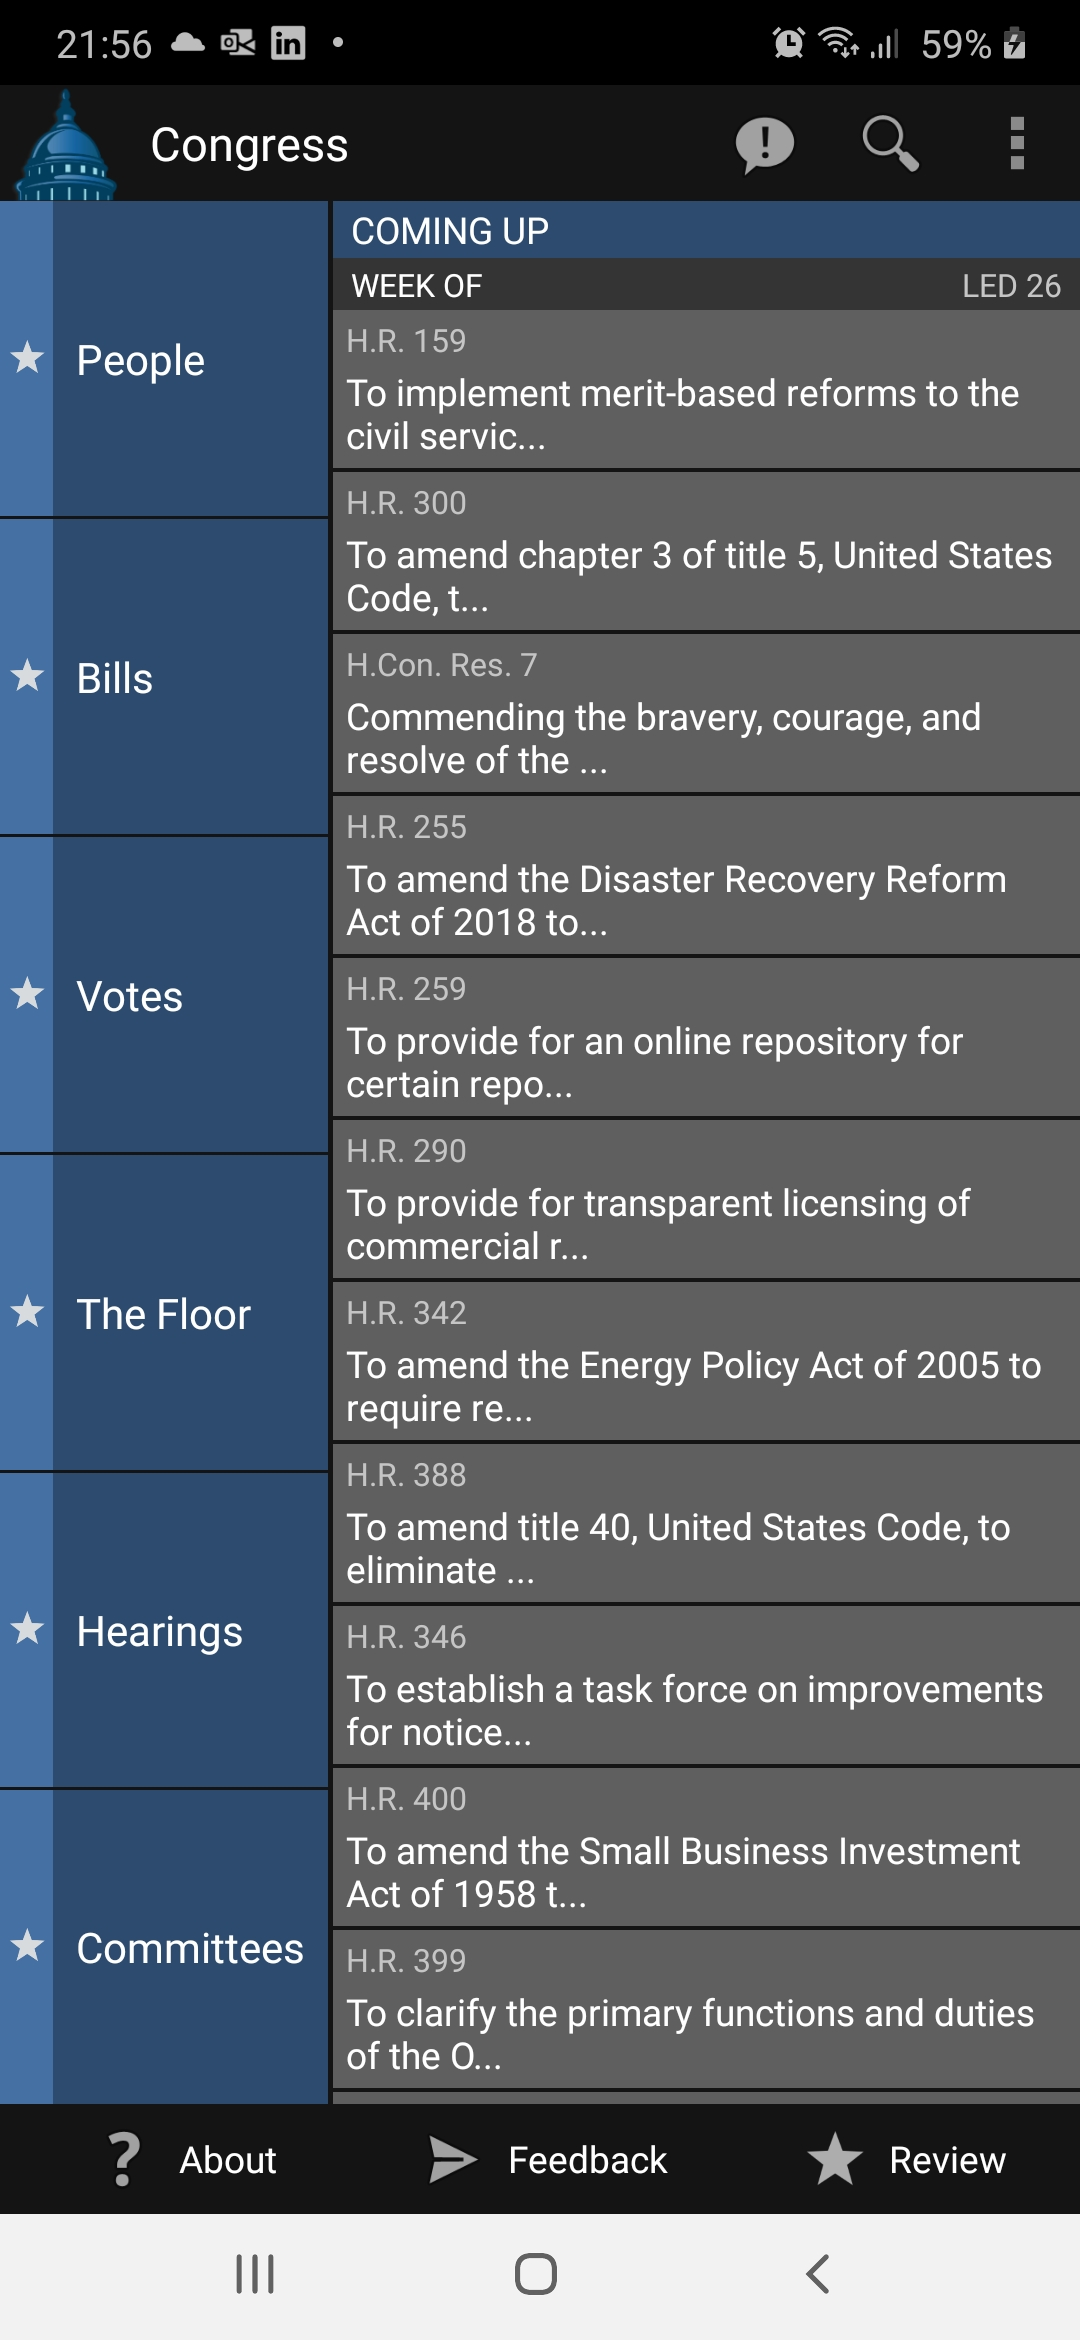
\includegraphics[width=0.4\linewidth]{congress_1}
	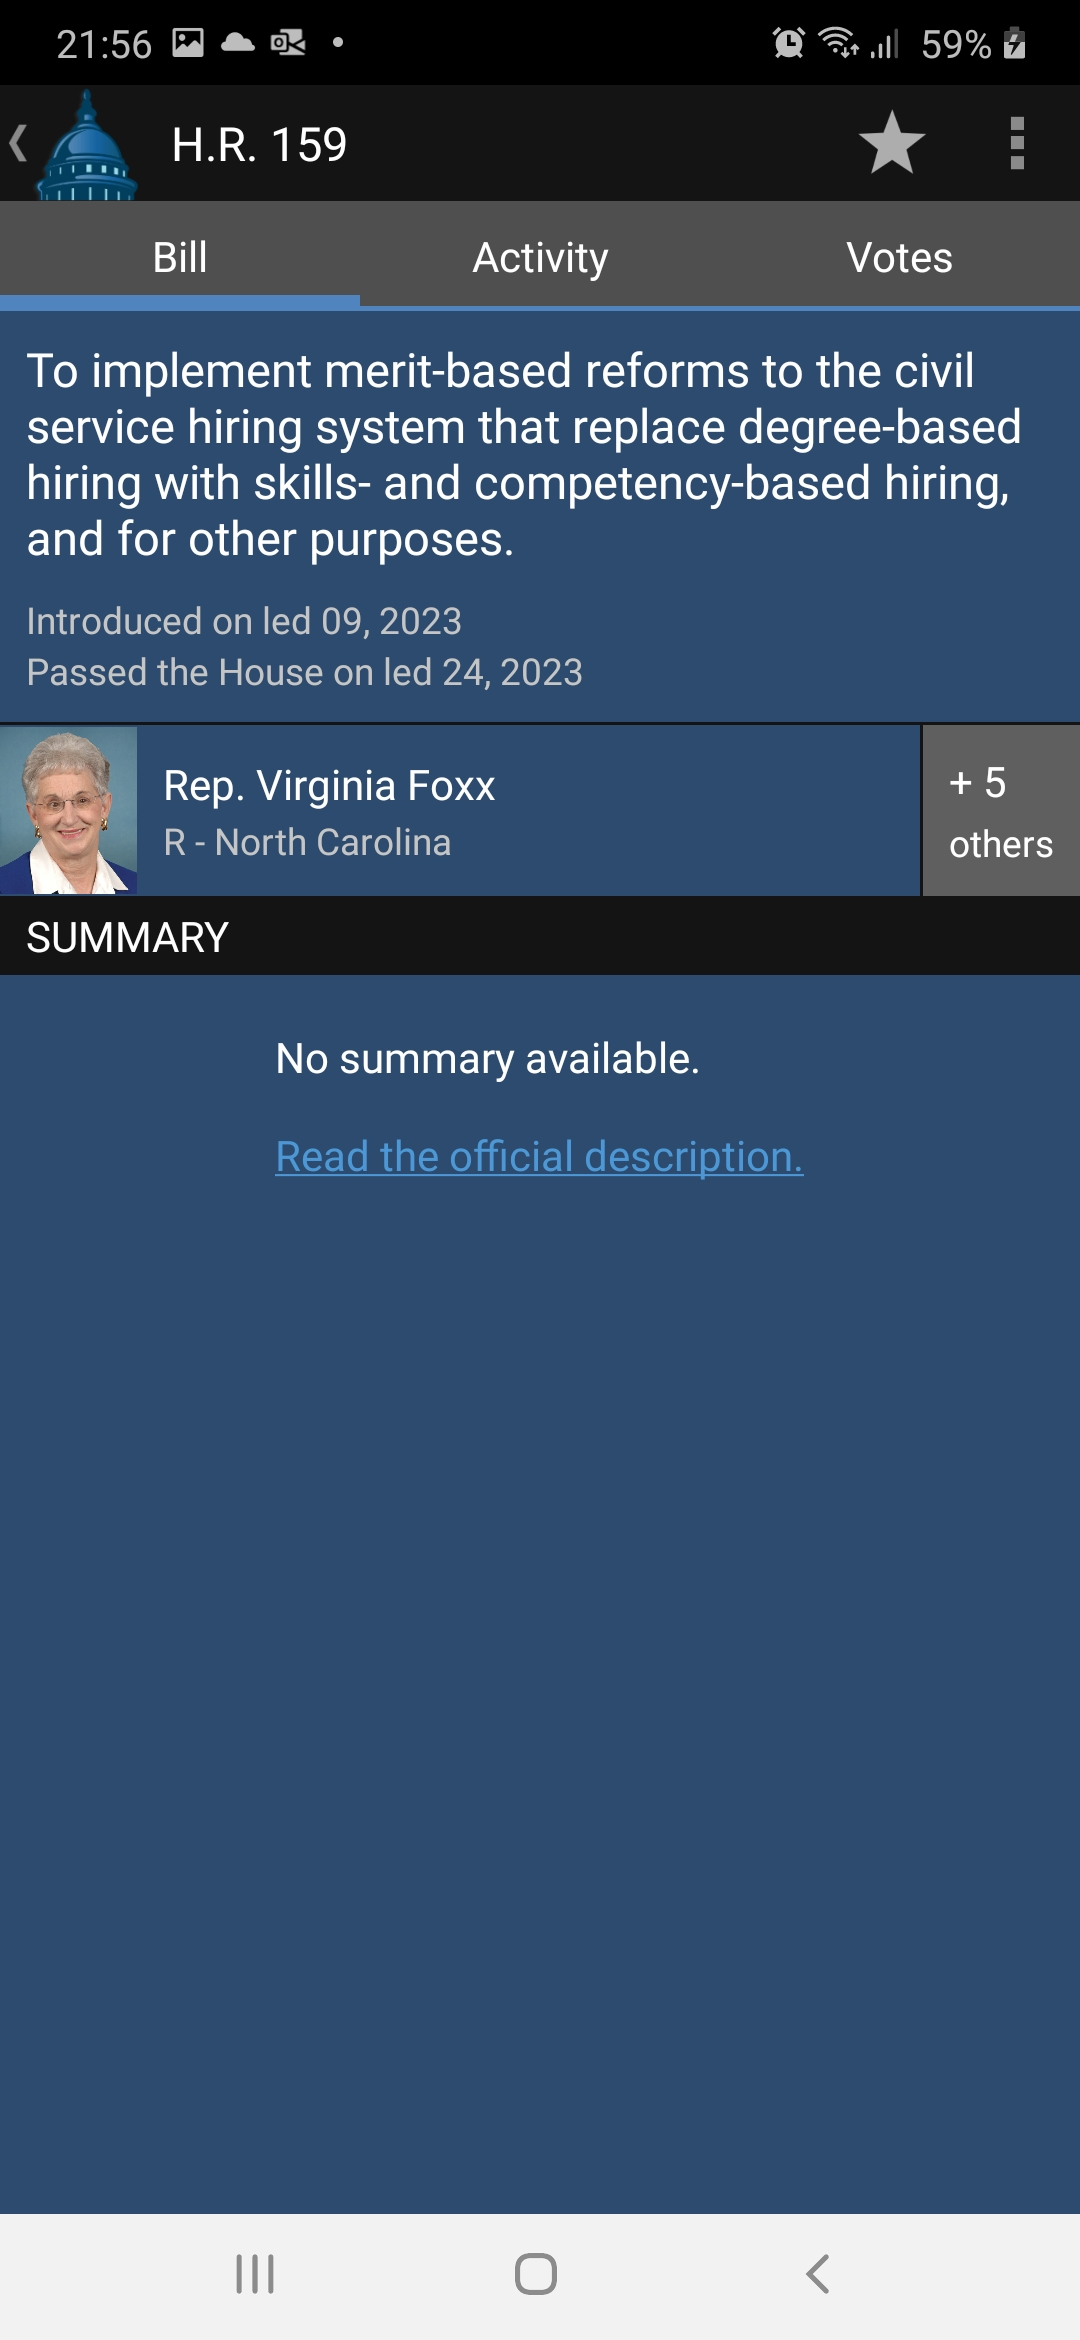
\includegraphics[width=0.4\linewidth]{congress_2}
	
	\caption{Android aplikace Congress \cite{congress}}
	\label{fig:congress}
\end{figure}

\subsection{Zhodnocení}
První dojem z této aplikace je to, že je velmi propracovaná z hlediska různorodosti poskytovaných informací. Přitom díky dobře navrženému uživatelskému rozhraní nepůsobí nepřehledně. Naopak působí velmi intuitivně. Z menu se lze dostat na jednotlivé hlavní obrazovky, které jsou dále rozděleny na taby. U návrhů zákonů lze snadno vidět výsledek jejich hlasování, jak hlasoval který \linebreak politik, proces schvalování návrhu a aktuální stav schvalování. Politiky lze vyhledávat podle jména, státu a příslušnosti ve Sněmovně nebo Senátu. Politiky a návrhy zákonů lze sledovat. Je také možné nastavit si notifikaci o změnách.

